\section{Discussão dos Resultados}
\label{sec:discussao}

Em linhas gerais, a placa de medição cumpriu o papel de aquisição e de
estimação embarcada, e os ensaios com as hélices, no 2º ensaio, ficaram próximos das curvas do fabricante. Os pontos que mais pesaram
nos resultados, discutidos a seguir, foram: as perdas descontadas no
torque das hélices; a incerteza da indutância do motor, medida por dois métodos que não
concordam; a faixa de corrente imposta pelo sensor Hall; o tempo e as falhas
de montagem da bancada; e a memória do microcontrolador, que condicionou a
forma de conexão com o computador.

\subsection{Coeficiente de Torque das Hélices}
\label{sec:discussao_helices}

O 1º ensaio das hélices ficou de \SIrange{19}{47}{\percent} acima da
curva do fabricante, e o 2º ensaio, entre \SI{-3}{\percent} e \SI{+9}{\percent}
(\autoref{sec:resultado_coef_aero_bancada}). Como a rotação e o torque
eletromagnético se repetiram entre os dois ensaios, a mudança veio
essencialmente das perdas a vazio descontadas, que no 2º ensaio
ficaram cerca do dobro das anteriores. O afastamento da bancada de objetos
próximos não alterou os resultados, o que indica que o escoamento ao redor da
hélice não era a causa da diferença.

A diferença entre os dois levantamentos de perdas tem explicações possíveis
que os dados não permitem separar: o primeiro usou o balanço de potência nos
registros de osciloscópio, enquanto o 2º ensaio usa o torque do próprio
observador; os controladores e as montagens mecânicas também eram outros.
Quando as perdas e o torque com carga vêm do mesmo observador, na mesma
montagem, um eventual viés do observador aparece nos dois e se cancela em boa
parte na subtração. Por isso o resultado indica que as perdas devem ser
levantadas nas mesmas condições do ensaio com hélice, mas não demonstra, por
si só, a exatidão absoluta do torque estimado. O residual de alguns pontos
percentuais na 17x10E é compatível com o viés do observador na simulação
(\autoref{sec:autotuning}) e com a extrapolação das perdas abaixo de
\SI{2500}{RPM}.

\subsection{Indutância do Motor}
\label{sec:discussao_indutancia}

Os dois métodos usados para obter a indutância divergem
(\autoref{sec:resultado_indutancia}). Uma possível causa é a frequência do
ensaio de ressonância, bem acima da frequência de chaveamento do controlador
em que o motor opera. Nessa faixa as perdas no ferro e as capacitâncias
parasitas do enrolamento passam a influenciar a medida, e o valor obtido pode
não representar a indutância vista pelo motor em operação. Além disso, o
circuito foi excitado diretamente pelo gerador de funções, sem amplificador de
potência, com correntes muito menores que as de operação. Já o ajuste aos
registros inclui os cabos e as ligações de cada montagem, e por isso pode variar de uma
montagem para outra.

\citeonline{hurley2013transformers} descrevem métodos mais adequados para
componentes magnéticos de potência, como a medição de impedância com
excitação senoidal em nível de potência, a medição com polarização em
corrente contínua e o método do degrau de tensão, que obtém a indutância pela
taxa de crescimento da corrente ($L = v\,\Delta t/\Delta i$) nas condições de
fluxo de operação. A aplicação de um desses métodos, com um amplificador de
potência ou com o próprio controlador do motor como fonte, permitiria
separar o que é do motor e o que é da montagem.

\subsection{Faixa de Medição de Corrente}
\label{sec:discussao_corrente}

A corrente máxima que a placa consegue medir é definida pelo sensor de
corrente escolhido, e não pelo conversor. Com o sensor Hall no núcleo
toroidal, a faixa linear do sensor corresponde a cerca de
$\pm\SI{60}{\ampere}$ por fase (\autoref{sec:same_sensor_corrente}); acima
disso a saída satura e a corrente lida fica menor que a real. Esse limite foi
suficiente para as hélices ensaiadas, mas restringe o uso da bancada com
hélices maiores ou com o motor em potência máxima. Ampliar a faixa depende de
trocar o sensor ou o núcleo, o que reduz a resolução nas correntes baixas.

\subsection{Montagem da Bancada e Falhas de Contato}
\label{sec:discussao_montagem}

Boa parte do tempo de ensaio foi consumida pela montagem e pela verificação
da bancada, e não pelos ensaios em si. A cada sessão era preciso refazer a
fiação de potência, dos sensores e da rede, e as falhas mais demoradas de
diagnosticar foram de contato: um canal de tensão de fase sem ligação à placa
de condicionamento, que aparecia como uma tensão flutuante, e um cabo de
corrente mal encaixado. Somou-se a isso o casamento entre correntes e tensões:
a sequência das correntes, como ligada, girava em sentido oposto ao das
tensões, e só a troca de duas fases com inversão de sinal levou a uma
potência elétrica coerente com a carga. Esses problemas não aparecem em
simulação e só foram identificados porque a telemetria trazia as grandezas
brutas de cada fase. Conectores com trava, um chicote fixo entre a placa de
condicionamento e o motor e uma verificação automática da sequência de fases
no início de cada ensaio reduziriam esse tempo.

\subsection{Memória do Microcontrolador e Conexão de Rede}
\label{sec:discussao_memoria}

A memória RAM do microcontrolador ficou quase toda ocupada, como mostra a
\autoref{fig:discussao_ram}. A maior parte não é da aplicação: a pilha de rede
e o \textit{driver} Ethernet, o núcleo do Zephyr e o registro de mensagens
somam cerca de dois terços do total. Da parte da aplicação, o maior consumo é
o dos \textit{buffers} de aquisição das fases, que recebem os lotes do
conversor por DMA em ping-pong.

\begin{figure}[H]
    \centering
    \caption{Ocupação da memória RAM do microcontrolador por componente do
    \textit{firmware}, em porcentagem dos \SI{128}{\kilo\byte} disponíveis.}
    \label{fig:discussao_ram}
    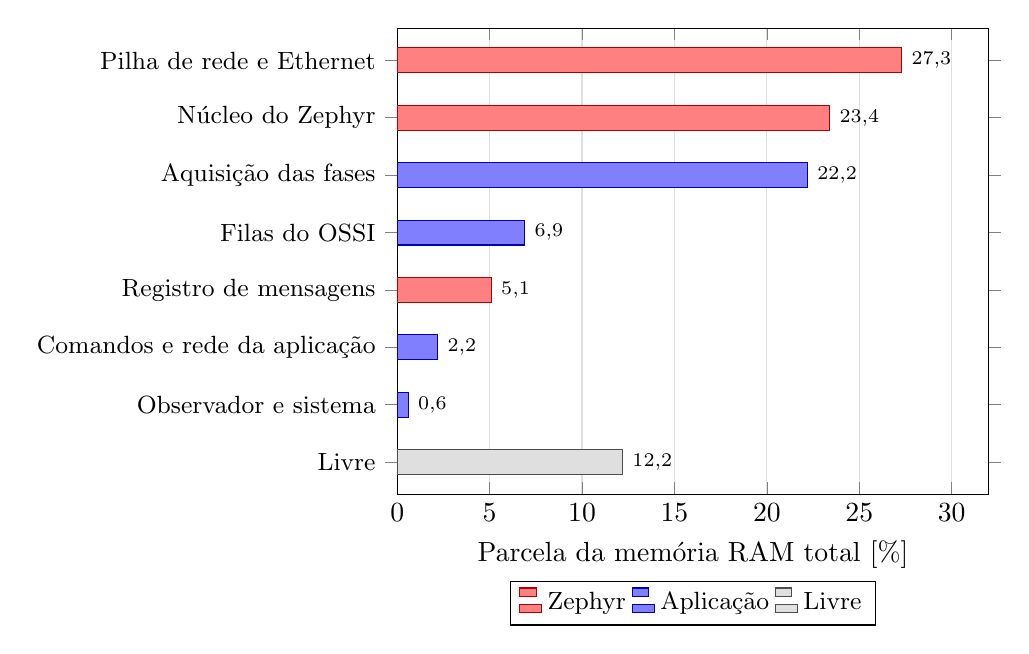
\begin{tikzpicture}
        \begin{axis}[
            xbar, bar width=9pt, bar shift=0pt, width=0.75\textwidth, height=7.5cm,
            legend style={at={(0.5,0)}, anchor=north, yshift=-1.1cm, legend columns=3, font=\small},
            xmin=0, xmax=32,
            xlabel={Parcela da memória RAM total [\%]},
            symbolic y coords={Livre, Observador e sistema, Comandos e rede da aplicação, Registro de mensagens, Filas do OSSI, Aquisição das fases, Núcleo do Zephyr, Pilha de rede e Ethernet},
            ytick={Livre, Observador e sistema, Comandos e rede da aplicação, Registro de mensagens, Filas do OSSI, Aquisição das fases, Núcleo do Zephyr, Pilha de rede e Ethernet},
            enlarge y limits=0.08,
            y tick label style={font=\small},
            nodes near coords={\pgfmathprintnumber[fixed, precision=1, use comma]{\pgfplotspointmeta}},
            nodes near coords style={font=\scriptsize},
            xmajorgrids, grid style={gray!25},
        ]
            \addplot[fill=red!50, draw=red!70!black] coordinates
                {(27.3,Pilha de rede e Ethernet) (23.4,Núcleo do Zephyr)
                 (5.1,Registro de mensagens)};
            \addplot[fill=blue!50, draw=blue!70!black] coordinates
                {(22.2,Aquisição das fases) (6.9,Filas do OSSI)
                 (2.2,Comandos e rede da aplicação) (0.6,Observador e sistema)};
            \addplot[fill=gray!25, draw=gray!60!black] coordinates
                {(12.2,Livre)};
            \legend{Zephyr, Aplicação, Livre}
        \end{axis}
    \end{tikzpicture}

    \fonte{Autor (2026), a partir do relatório de memória do Zephyr.}
\end{figure}

Com essa ocupação, não sobrou espaço para um servidor DHCP na placa, que
exigiria contextos de rede, \textit{sockets} e \textit{buffers} adicionais. A
solução adotada foi o endereçamento estático na faixa \textit{link-local}: a placa tem endereço fixo e o computador precisa ser
configurado manualmente com um endereço da mesma sub-rede. A telemetria é
enviada por \textit{broadcast} UDP, de modo que a placa não precisa conhecer o
endereço do computador, mas o sistema operacional classifica essa rede, sem
\textit{gateway}, como não identificada e aplica o perfil mais restritivo do
\textit{firewall}, o que exige regras de entrada para as portas da telemetria e
dos comandos. É um arranjo funcional, mas pouco prático: a cada troca de
computador ou de interface de rede a configuração precisa ser refeita. Liberar
memória, por exemplo reduzindo o registro de mensagens e os \textit{buffers} da
pilha de rede, ou migrar para um microcontrolador com mais RAM, permitiria
incluir o DHCP ou um protocolo de descoberta automática.
